\newpage
\section{Design}
\subsection{Anforderungen}
Das Design des Antennensystems wird für einen Anwendungsfall im Freiraum dimensioniert. Die Distanz zwischen Sender und Empfänger soll 10 Meter betragen. Das Übertragungsmedium ist Luft, kann aber idealisiert als Vakuum angenommen werden. Das System soll isotrop abstrahlen und der Gewinn der Empfangsantenne kann mit einem Faktor  1 angenommen werden. Die Antenne soll symmetrisch gespiesen werden und im 2.4 GHz ISM Band arbeiten. Als Quelle dient ein Bluetooth Low Energie Texas Instruments CC2541 Chip mit 0 dBm als Sendeleistung. Als Designkriterien wird eine $S_{11}$ Dämpfung von -10 dB mit einer Bandbreite von midestens 100 MHz gefordert und eine Reserve von 6 dB soll in das Linkbudget eigerechte werden. Die Abbildung \ref{fig:DesignAusgangslage} zeigt die Welsentlichen Punkte der Design Anforderungen.

%%%%%%%%%%%%%%%%%%%%%%%%%%%%%%%%%
\begin{figure}[h]
\begin{center}
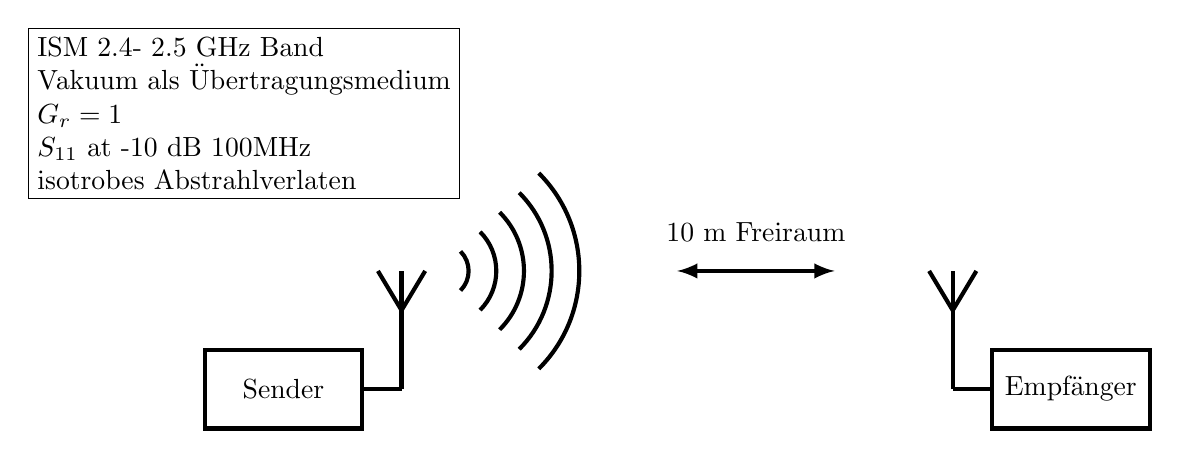
\begin{tikzpicture}
	\draw[line width=1.5pt](0, 0) rectangle (2, 1) node[pos=0.5] {Sender};
	\draw[line width=1.5pt] (2, 0.5) -- (2.5, 0.5);%zuleitung
	\draw[line width=1.5pt] (2.5, 0.5) -- (2.5, 1.5);%Antennenmast
	\draw[line width=1.5pt] (2.5, 1.5) -- (2.2, 2);%Antenne
	\draw[line width=1.5pt] (2.5, 1.5) -- (2.8, 2);
	\draw[line width=1.5pt] (2.5, 1.5) -- (2.5, 2);
	
	\draw[line width=1.5pt, <->, >=latex](6, 2)  -- (8, 2) node at (7, 2.5) {10 m Freiraum};
	
	\draw[line width=1.5pt] (9.5, 0.5) -- (10, 0.5);%zuleitung
	\draw[line width=1.5pt] (9.5, 0.5) -- (9.5, 1.5);%Antennenmast
	\draw[line width=1.5pt] (9.5, 1.5) -- (9.2, 2);%Antenne
	\draw[line width=1.5pt] (9.5, 1.5) -- (9.8, 2);
	\draw[line width=1.5pt] (9.5, 1.5) -- (9.5, 2);
	\draw[line width=1.5pt,decorate,decoration=expanding waves](3, 2) -- (5, 2);
	\draw[line width=1.5pt](10, 0) rectangle (12, 1) node[pos=0.5] {Empfänger};
	\node[draw,align=left] at (0.5,4) {ISM 2.4- 2.5 GHz Band\\ Vakuum als Übertragungsmedium\\ $G_{r} =1$\\ $S_{11}$ at -10 dB 100MHz \\ isotrobes Abstrahlverlaten};
\end{tikzpicture}
\end{center}
\caption{Design Ausgangslage}
\label{fig:DesignAusgangslage}
\end{figure}
%%%%%%%%%%%%%%%%%%%%%%%%%%%%%%%%%%%%%%%%%%

%\subsection{Technische Spezifikationen und Anforderungsliste}
%%\todo{Anforderungskatalogs mit Fest-, Mindest- \& Wunschforderungen}
%\begin{itemize}
%\item Geräte Connect 1
%\item Materialien des Gehäuse ABS Kusnstoff
%\item Volumen des Antennensystems
%\item Wirkungsradius 10m im Freiraum
%\item Richtcharakteristik isotroph
%\item Polarisation linear
%\item Antennen Wirkungsgrad ist zubestimmen
%\item Antennen Gewinn gleich wir der Abstrahl Wirkungsgrad
%\item minimaler Empfangspegel am Transceivers
%\item Transceivers Baustein Texas Instruments CC2541
%\item Sendeleistung
%\item $S_{11} \leq$ 10 dB
%\end{itemize}

\begin{table}[htb]
 \centering
\begin{tabular}{lccc}\toprule 
Nr. & Anforderung & Beschreibung & Wert   \\ 
001 & f & ISM Frequenzbereich  & 2.4-2.5 GHz  \\ 
002 & f & Handgerät lxbxh & 142x88x23 [mm]    \\  
003 & f &  Speisung des Antennensystems & symmetrisch  \\  
004 & f & Reflexionskoeffizient der Antenne  at -10B & 100 MHz  \\ 
005 & f & Funkdistanz, Arbeitsradius & 10m   \\ 
006 & f & Linkbudget Reserve & 6dB   \\ \bottomrule
  \end{tabular}
  \caption{Anforderungen an das Bluetooth Antennensystem}
  \label{AnforderungenAntenneSystem}
\end{table} 



\subsection{Analyse mit bekannten Modellen}
\subsection{Neue Design Ansätze}